\documentclass[12pt, letterpaper]{article}
\usepackage[utf8]{inputenc}
\usepackage[portuguese]{babel}
\usepackage{graphicx}
\usepackage{listings}
\usepackage{xcolor}
\lstset { %
    language=C++,
    basicstyle=\ttfamily,
    keywordstyle=\color{blue}\ttfamily,
    stringstyle=\color{red}\ttfamily,
    commentstyle=\color{green}\ttfamily,
    morecomment=[l][\color{magenta}]{\#}
    extendedchars=true,
    inputencoding=utf8,
    literate=%
    {á}{{\'a}}1
    {ã}{{\~a}}1
    {č}{{\v{c}}}1
    {ď}{{\v{d}}}1
    {é}{{\'e}}1
    {ě}{{\v{e}}}1
    {í}{{\'i}}1
    {ň}{{\v{n}}}1
    {ó}{{\'o}}1
    {ř}{{\v{r}}}1
    {š}{{\v{s}}}1
    {ť}{{\v{t}}}1
    {ú}{{\'u}}1
    {ů}{{\r{u}}}1
    {ý}{{\'y}}1
    {ž}{{\v{z}}}1
    {Á}{{\'A}}1
    {Č}{{\v{C}}}1
    {Ď}{{\v{D}}}1
    {É}{{\'E}}1
    {Ě}{{\v{E}}}1
    {Í}{{\'I}}1
    {Ň}{{\v{N}}}1
    {Ó}{{\'O}}1
    {Ř}{{\v{R}}}1
    {Š}{{\v{S}}}1
    {Ť}{{\v{T}}}1
    {Ú}{{\'U}}1
    {Ů}{{\r{U}}}1
    {Ý}{{\'Y}}1
    {Ž}{{\v{Z}}}1
}
\title{Prova teórica II}
\author{Matheus Filipe dos Santos Reinert - 18100033}
\date{\today}

\begin{document}
    \maketitle
    x = (0 + 3 + 3) \% 3 = 0
    \begin{enumerate}
        \item
        \begin{enumerate}
\item{O fator de balanceamento é dado pela diferença de altura entre a subárvore da esquerda e da direita. 
A cada nó que percorremos partindo da raíz a altura diminui 1, por exemplo a altura de B é h, logo a altura 
de z será h + 1, então temos:\newline\newline x: altura(y) - altura(D) = (h + 2) - (h + 1) = 1\newline y: altura(A) 
- altura(z) = (h + 1) - (h + 1) = 0 \newline z: altura(B) - altura(C) = h - h = 0}

\item{Como a altura de D é h + 1, o desequilíbrio ocorre no nó y\newline\newline Inserindo o nó N no nó C:\newline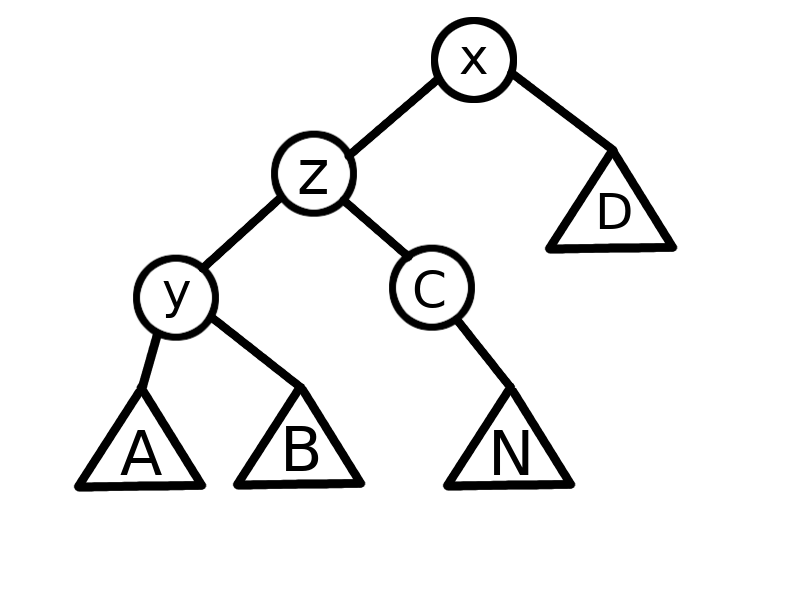
\includegraphics{arvore1.png}\newline\newline\newline\newline}
        \end{enumerate}
        
        \item
\begin{lstlisting}
//! Quantos nós da árvore estão cheios
template <class T, int M>
int BTreeNode<T, M>::conta_nos_cheios(BTreeNode<T, M> *node) {
    // Caso específico para ponteiro nulo
    if (node == nullptr)
        return 0;

    int total = 0;  // total de nós cheios
    bool full = true;  // se o nó está cheio
    // Verifica se o nó está cheio, se estiver soma 1 ao
    // total se não ignora
    for (int i = 0; i < M - 1; i++)
        if (node->keys[i] == NULL)
            full = false;
    if (full)
        total++;
    // Repetimos isso recursivamente para todos os nós
    for (int i = 0; i < M; i++)
        total += conta_nos_cheios(node->pointers[i]);

    return total;
}
\end{lstlisting}
    \item
    \begin{enumerate}
        \item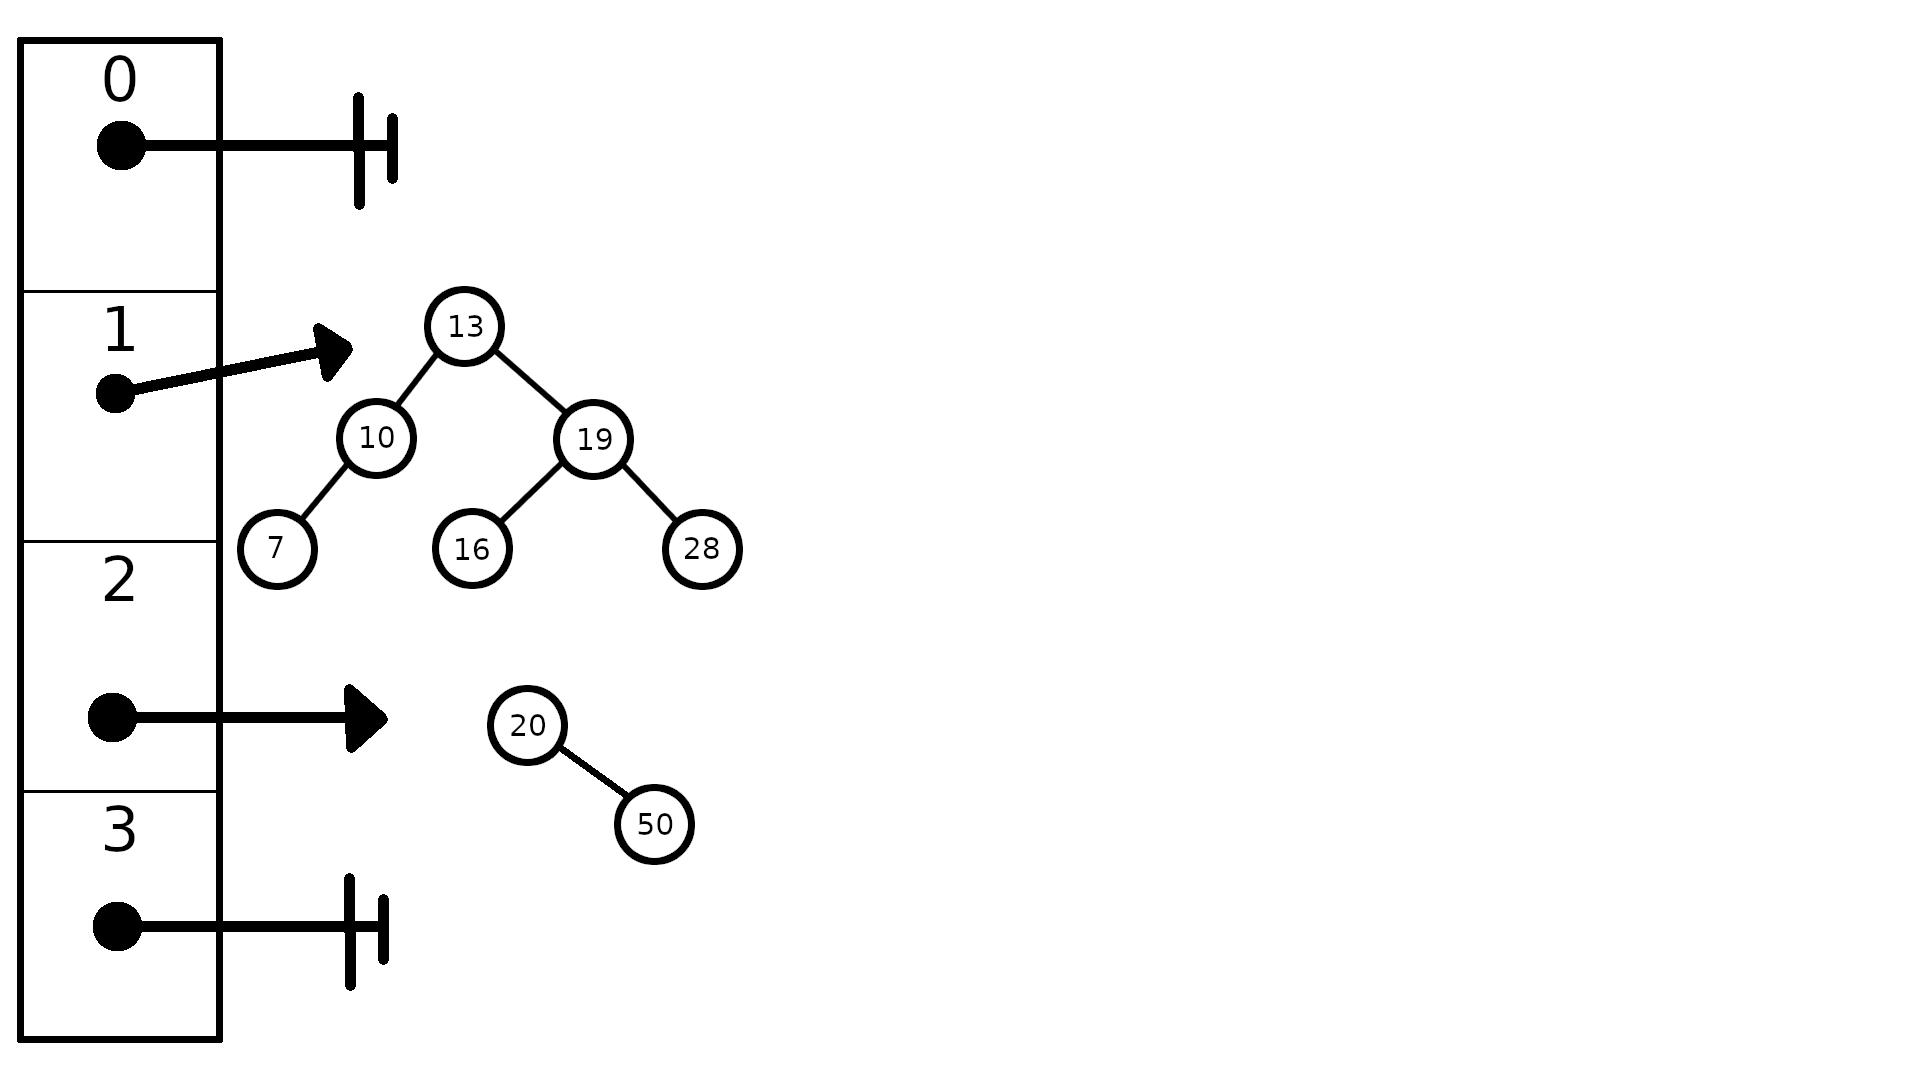
\includegraphics{questao3a.png}
        \item
        Método transformar hash em lista ordenada:
        \begin{lstlisting}
template <typename T>
LinkedList<T> Hash<T>::ordena() {
    auto lista = new LinkedList<T>();
    for (int i = 0; i < S; i++) {
        auto elementos = tabela[i].in_order();
        for (int j = 0; j < tabela[i].size(); j++)
            lista->insert_sorted(elementos[j]);
    }

    return lista;
}
        \end{lstlisting}
    \item
    Método maior elemento do hash:
\begin{lstlisting}  
template<typename T>
T Hash<T>::maximo() {
    // Os máximos de cada depósito
    T maximos[S];

    for (int i = 0; i < S; i++) {
        auto arvore = tabela[i];
        Node *aux = arvore.root();
        // Percorremos até o elemento mais a direita
        while (aux->right() != nullptr)
            aux = aux->right();
        maximos[i] = aux->data();
    }
    // Retorna o máximo da lista
    return std::max(maximos);
}
\end{lstlisting}
    \item {
Para o algoritmo do item b, temos que para criarmos um array com os elementos in order a complexidade é O(n), com n sendo o número de elementos
da árvore, e para inserirmos em ordem na linked list também temos complexidade O(n), pois precisamos percorrer a lista até acharmos onde colocar,
porém inserção em linked list é de ordem O(1) mas o O(n) acaba pesando muito mais que o O(1), então como resultado tempos complexidade O(n²).\newline
Já para o algoritmo do item c, como já sabemos onde está o maior elemento de cada depósito do hash só precisamos percorrer até ele na árvore, o que é complexidade
O(1), inserção no array maximos também é O(1), porém no fim precisamos comparar os resultados de cada depósito o que no pior caso é O(N-1),
N sendo o número de elementos para comparar, neste exercício N=4, como O(N-1) acaba pesando mais que 2 O(1), temos que a complexidade é O(N-1).
    }
    \end{enumerate}
    \item
    \begin{enumerate}
        \item {
            Como é um algoritmo recursivo temos que a variável pivô, para cada chamada do método, é:
            \newline\newline
            1ª: 30\newline
            2ª: 20\newline
            3ª: 40\newline
            4ª: 70\newline
            5ª: 50\newline
            6ª: 100\newline
            7ª: 90\newline\newline
        }
        \item {
            Para cada partição temos que o conteúdo do array é:\newline\newline
            1ª: [20, 10, 30, 40, 70, 80, 90, 100, 60, 50]\newline
            2ª: [10, 20, 30, 40, 70, 80, 90, 100, 60, 50]\newline
            3ª: [10, 20, 30, 40, 70, 80, 90, 100, 60, 50]\newline
            4ª: [10, 20, 30, 40, 50, 60, 70, 100, 80, 90]\newline
            5ª: [10, 20, 30, 40, 50, 60, 70, 100, 80, 90]\newline
            6ª: [10, 20, 30, 40, 50, 60, 70, 90, 80, 100]\newline
            7ª: [10, 20, 30, 40, 50, 60, 70, 80, 90, 100]\newline
        }
    \end{enumerate}
    \end{enumerate}
\end{document}